% DRAFTING-ONLY RESULTS TEXT.
% All numerical values and figures in this file are based on synthetic,
% literature-informed data. Replace them with measured multi-seed ns-3 and
% offline-RF results before submission.

\section{Illustrative Results and Discussion}
\label{sec:diss}

\noindent\textbf{Drafting-only notice:} The figures and numerical values in
this temporary section illustrate the intended presentation and discussion.
They are not results obtained from ns-3 or a trained RF model and must be
replaced before performance claims are made.

\subsection{System-Level ISAC Sensing Performance}

Fig.~\ref{fig:isac-sensing-performance} illustrates the relationship between
sensing range, empirical UE-detection probability, and conditional
localisation RMSE. Each range bin contains 400 synthetic observations, and the
error bars represent 95\% confidence intervals. Detection remains close to
one below 300~m, decreases to approximately 0.87 at 500~m, crosses 0.5 near
700~m, and falls below 0.15 at 1~km. At the same time, the conditional
localisation RMSE increases from approximately 1.4~m at 100~m to 7.4~m at
500~m and 17.3~m at 1~km. This behaviour follows the $r^{-4}$ attenuation of
the monostatic echo SNR: increasing range both lowers the probability of a
successful observation and increases the variance of a detected position.
The RMSE is reported only when at least 20 detections are available in a range
bin, thereby avoiding an unstable estimate based on a few unusually strong
echoes. For this temporary example, a 30-dB effective aggregate sensing loss
is used because the uncalibrated value $L_s=1$ produces nearly deterministic
detection throughout the compact area. The final figure must therefore be
regenerated after the effective sensing power/loss is calibrated and frozen.

\begin{figure}[!t]
    \centering
    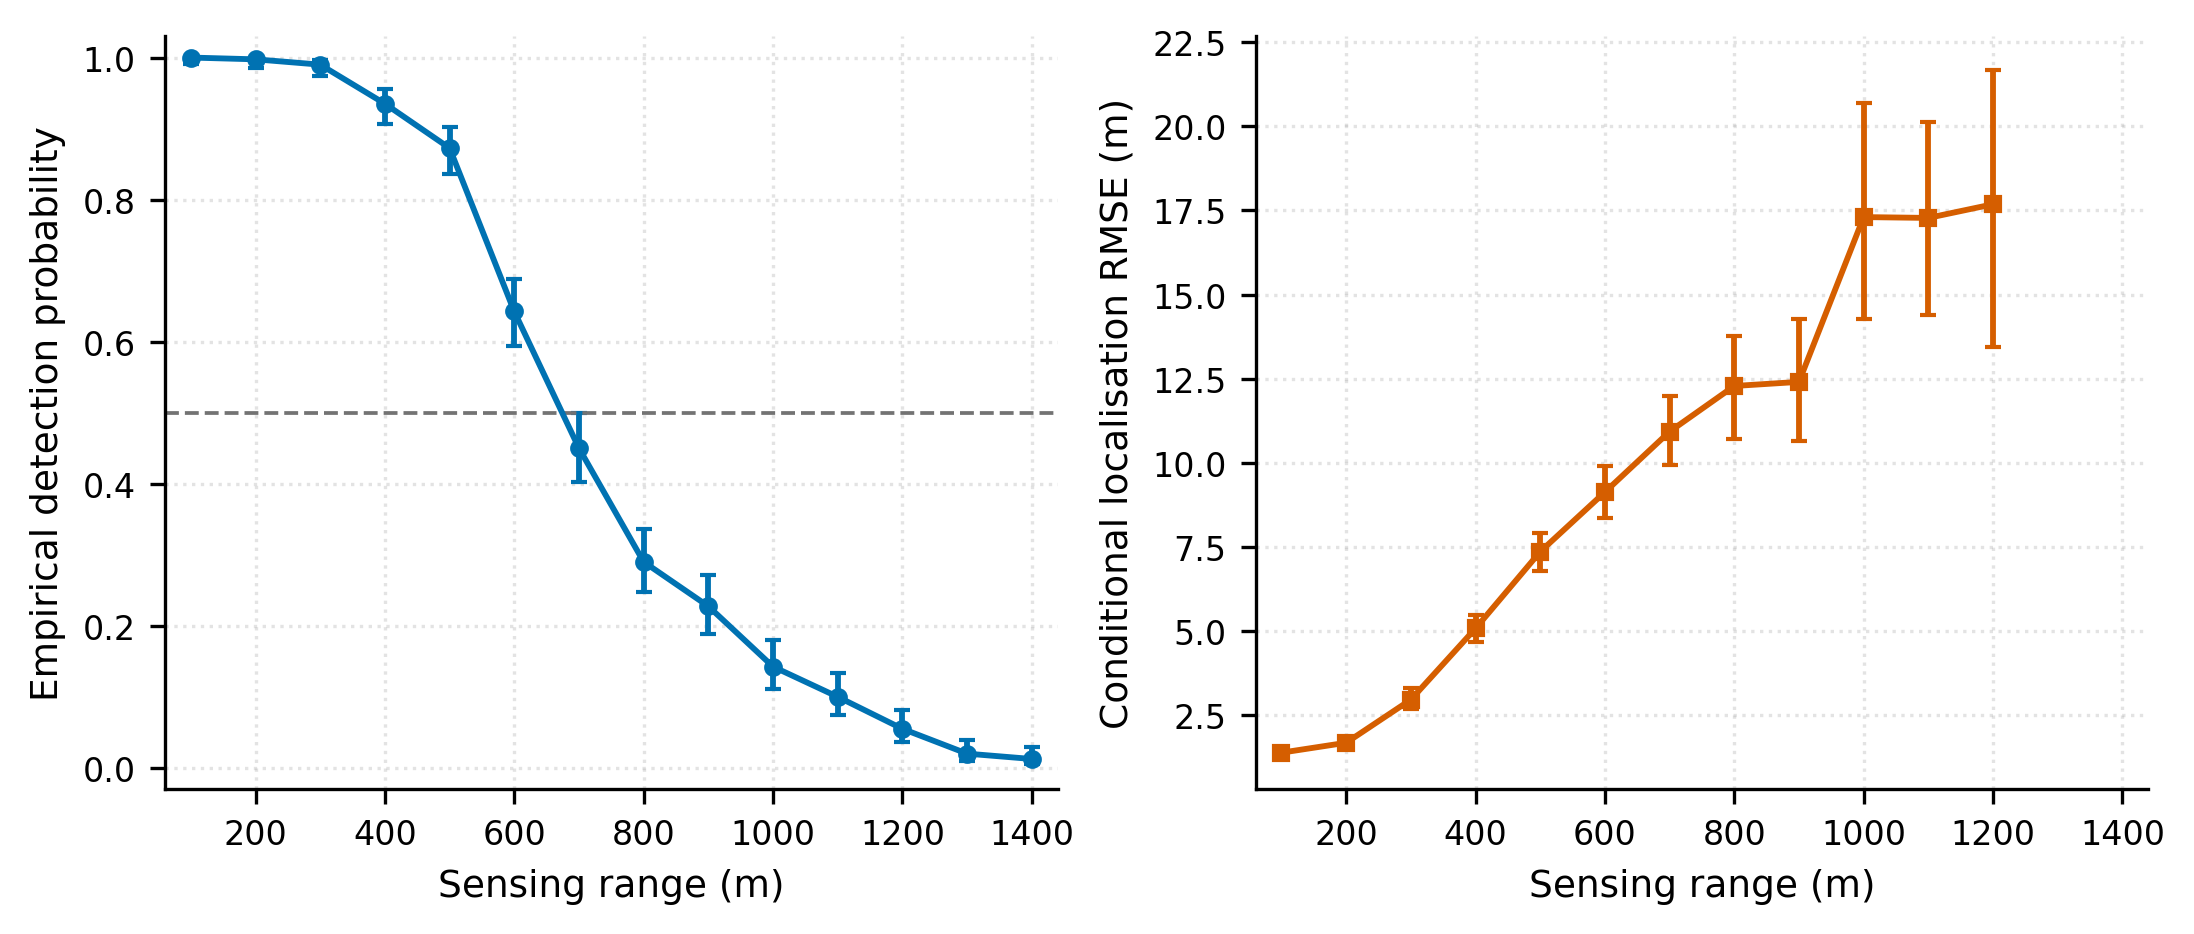
\includegraphics[width=\linewidth]
    {results/plots/sample-png/isac-sensing-performance.png}
    \caption{UE-detection probability and conditional localisation RMSE as a
    function of sensing range. The displayed values are synthetic and use a
    temporary 30-dB effective aggregate sensing loss.}
    \label{fig:isac-sensing-performance}
\end{figure}

\subsection{Future Repositioning-Demand Prediction}

Fig.~\ref{fig:rf-prediction-performance} presents the intended evaluation of
the RF repositioning-demand predictor for horizons of 2, 5, and 10~s. The
left-hand panel shows precision--recall curves, which are more informative
than accuracy because positive repositioning-hotspot cells form a minority
class. The right-hand panel reports the mean precision, recall, and F1 score
over ten synthetic test seeds at thresholds selected independently of those
test samples. At 2~s, the short-term spatial state remains highly informative,
resulting in precision, recall, and F1 values of approximately 0.95, 0.91, and
0.93, respectively. At 5~s, the F1 score decreases to approximately 0.78 as
UE motion and service-state transitions introduce greater uncertainty. At
10~s, recall remains comparatively high, but precision decreases, producing
an F1 score of approximately 0.63. This result pattern illustrates the
expected cost of predicting farther into the future: a lower decision
threshold can preserve hotspot recall but also selects more false-positive
grid cells. In the final experiment, these metrics must be computed using
seed-disjoint training, validation, and testing sets, and interpreted together
with measured hotspot lifetimes and grid-label transition rates.

\begin{figure}[!t]
    \centering
    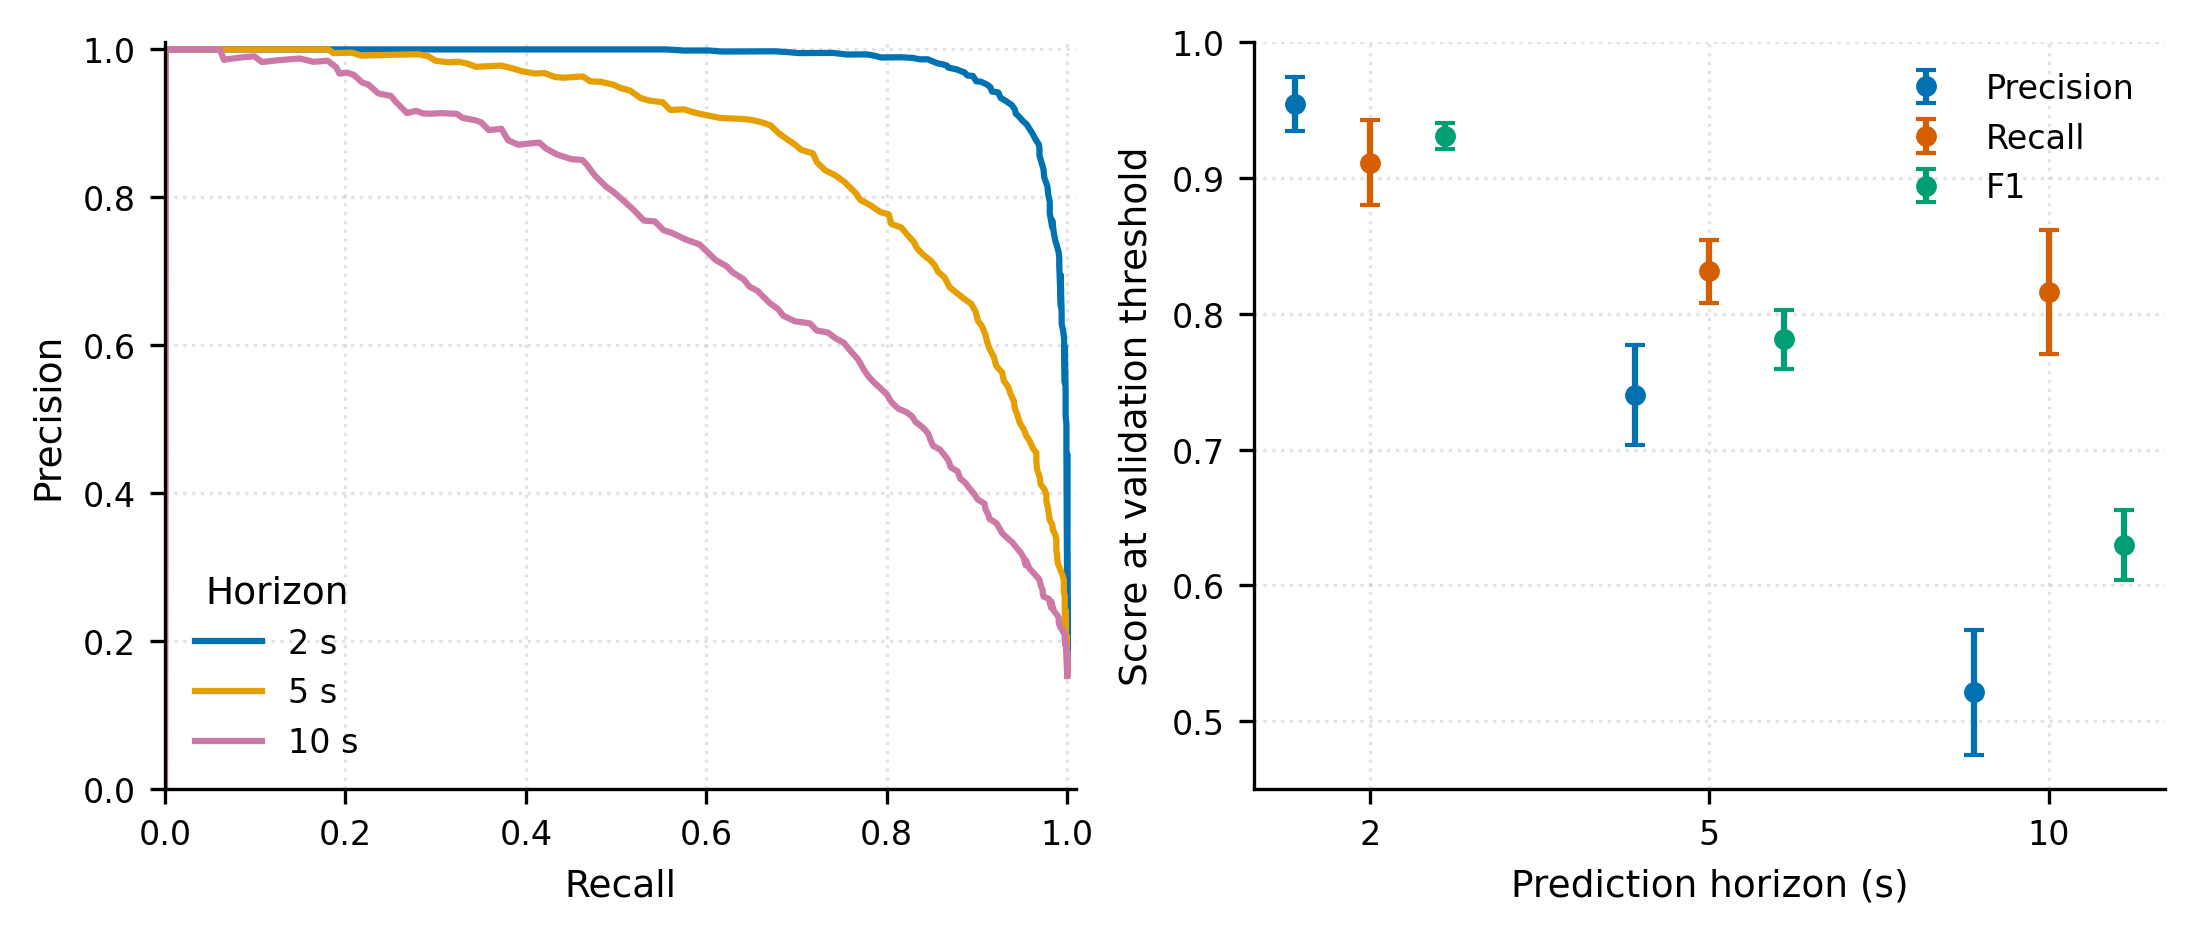
\includegraphics[width=\linewidth]
    {results/plots/sample-png/rf-prediction-performance.png}
    \caption{Precision--recall behaviour and grid-cell classification scores
    for future repositioning-demand prediction. The displayed RF scores are
    synthetic placeholders for the final seed-disjoint evaluation.}
    \label{fig:rf-prediction-performance}
\end{figure}

\subsection{End-to-End Controller Comparison}

Fig.~\ref{fig:controller-comparison} compares the static-UAV,
oracle-position reactive, ISAC-sensed reactive, and ISAC--RF predictive
controllers for total loads of 80, 90, and 100 UEs. Faint points represent ten
synthetic seed outcomes, while the markers and error bars show the mean and
95\% confidence interval. All methods degrade as the UE load increases,
because more UEs compete for finite TN and UAV resources. For the middle
90-UE case, the static baseline obtains a fifth-percentile downlink throughput
of approximately 0.032~Mbit/s, an outage-time fraction of 0.39, and a
persistent repositioning-demand fraction of 0.32. Oracle-reactive K-means
improves these values to approximately 0.101~Mbit/s, 0.15, and 0.10,
respectively, showing the potential benefit of correctly repositioning UAVs
towards unresolved demand. Replacing true coordinates with fused ISAC
estimates introduces missed detections and localisation error; consequently,
the ISAC-reactive method reaches approximately 0.082~Mbit/s throughput and
0.23 outage. The predictive controller partially closes this gap, reaching
approximately 0.094~Mbit/s and reducing outage to 0.18 by initiating movement
towards likely future demand. This comparison separates three effects:
movement gain is measured by static versus oracle-reactive control, sensing
cost by oracle-reactive versus ISAC-reactive control, and prediction gain by
ISAC-reactive versus ISAC--RF control. The final paper must replace these
values with aligned multi-seed simulation results before calculating relative
improvements.

\begin{figure*}[!t]
    \centering
    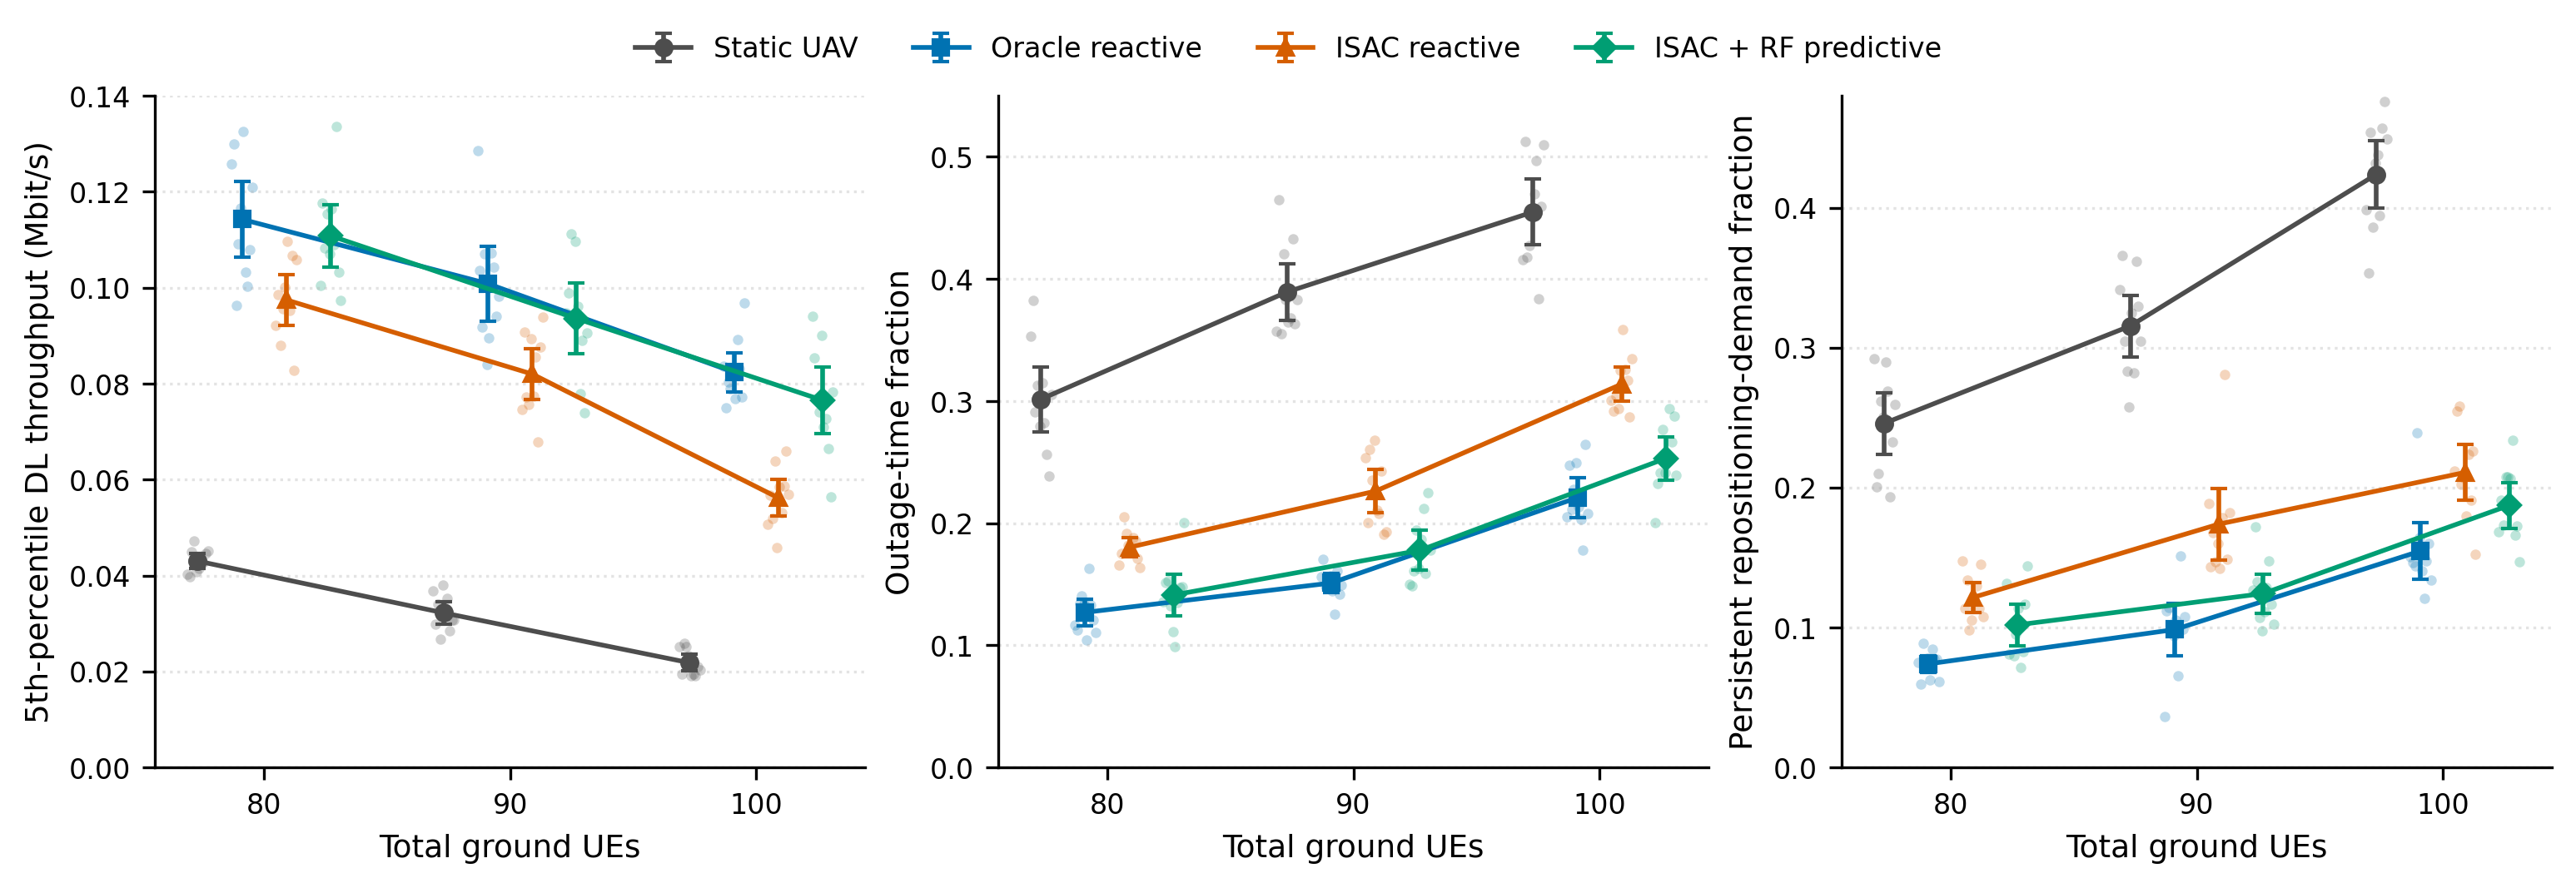
\includegraphics[width=0.98\textwidth]
    {results/plots/sample-png/controller-comparison.png}
    \caption{Comparison of fifth-percentile downlink throughput, outage-time
    fraction, and persistent repositioning-demand fraction across UE loads.
    Faint points denote synthetic seed outcomes, and error bars show synthetic
    95\% confidence intervals.}
    \label{fig:controller-comparison}
\end{figure*}

Fig.~\ref{fig:controller-dynamics} complements the run-level comparison by
showing how persistent repositioning demand evolves during the 90-s
middle-load experiment. The first service assessment occurs when the
controller starts at 12~s. Consequently, a connected weak-service UE cannot
enter the movement-target set before approximately 18~s, after satisfying the
6-s persistence interval. A UE initially classified as UNKNOWN may require
approximately 24~s because it must first complete the 6-s UNKNOWN timeout and
then the persistence interval. The demand fraction therefore begins to rise
between approximately 18 and 24~s rather than immediately at controller
activation. The static-UAV baseline stabilises near 0.31 because its UAVs do
not move towards unresolved demand. The reactive methods begin reducing
demand only after target formation and a physically plausible UAV travel
interval. Oracle-reactive control converges near 0.08, whereas sensing misses
and localisation uncertainty leave the ISAC-reactive controller with a higher
residual near 0.13. The predictive controller can begin travelling towards a
region expected to satisfy the future movement criterion before the reactive
target set fully develops; it therefore reduces demand earlier than
ISAC-reactive control and stabilises near 0.10. This time-domain view helps
verify that the improvement follows the implemented state transitions and UAV
motion, rather than occurring instantaneously. In the final analysis, actual
target-formation and UAV-arrival events from the decision and assignment
traces should be overlaid on the measured curves.

\begin{figure}[!t]
    \centering
    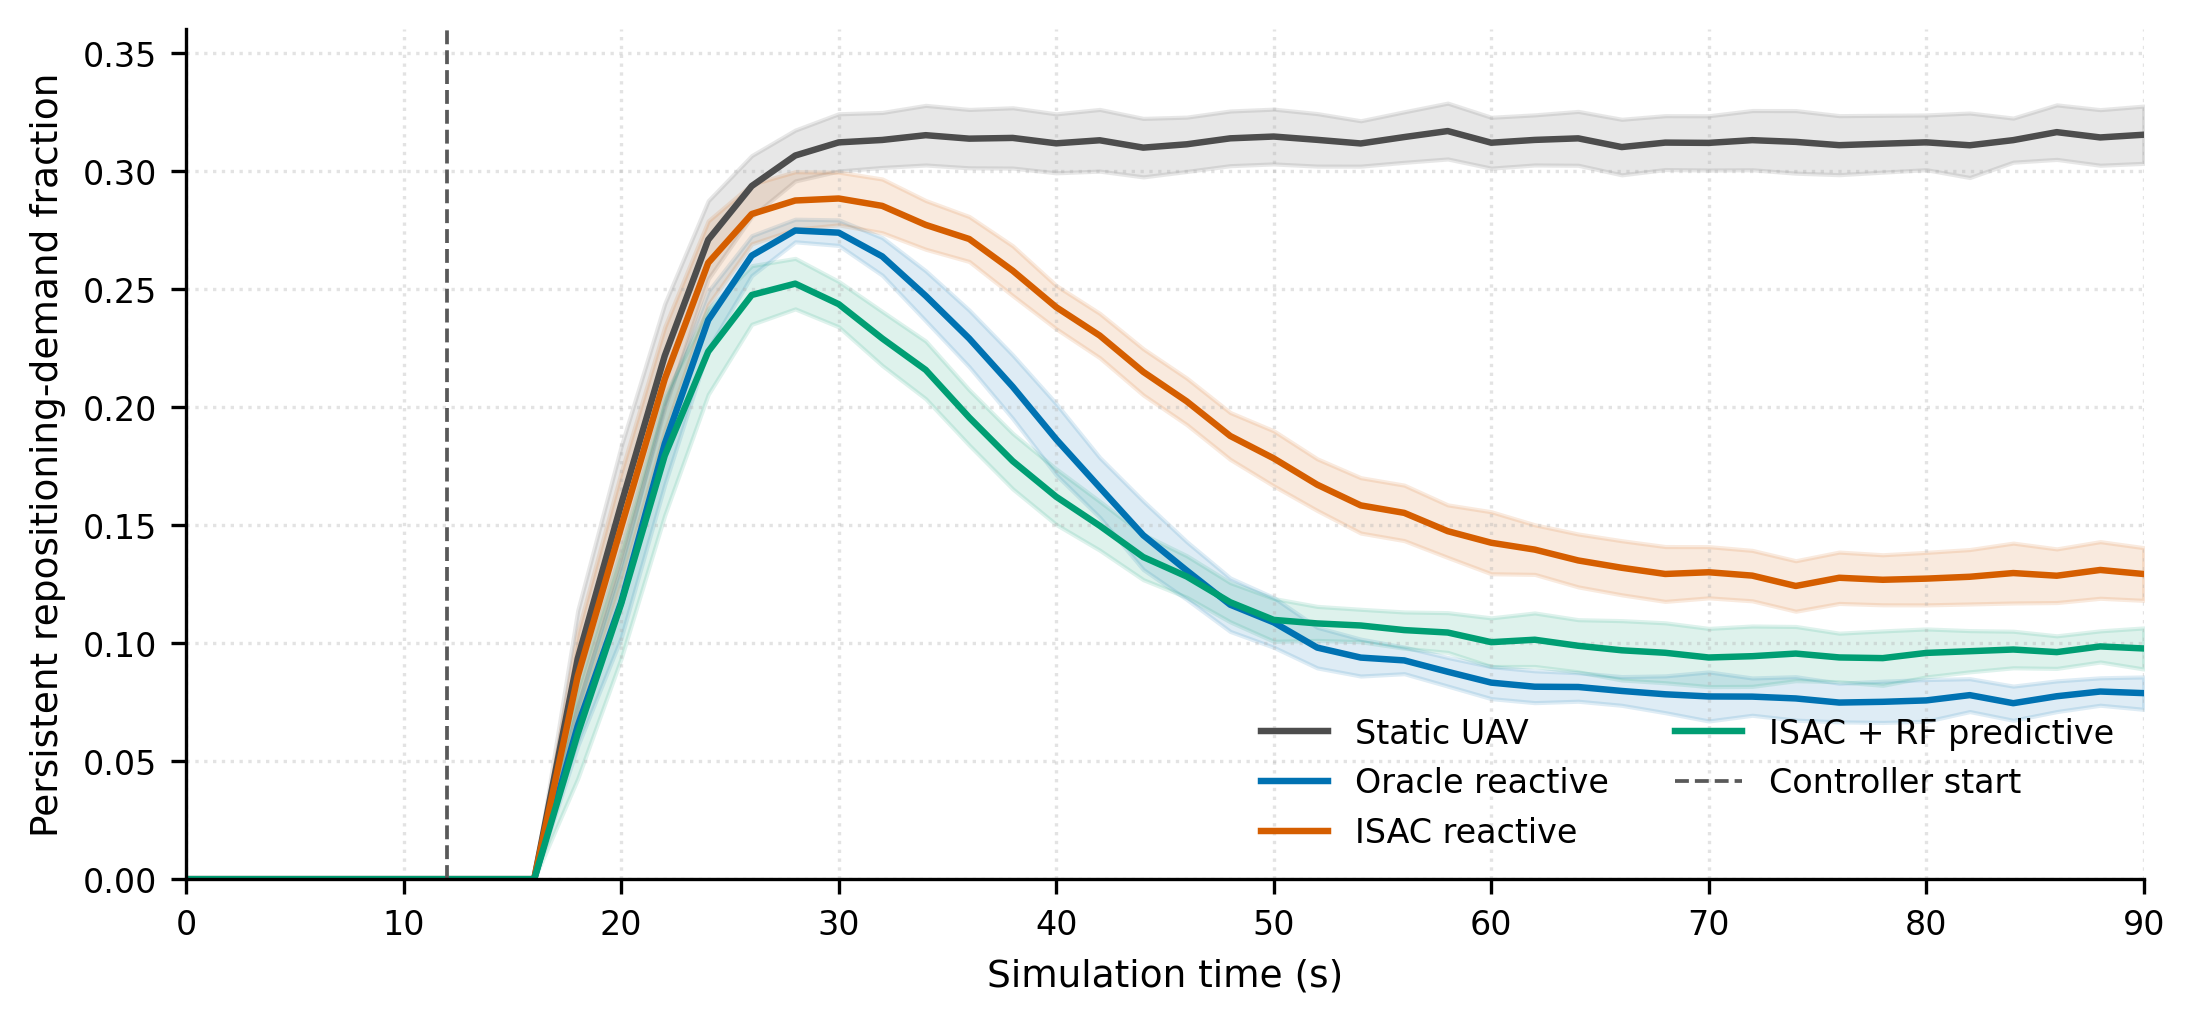
\includegraphics[width=\linewidth]
    {results/plots/sample-png/controller-dynamics.png}
    \caption{Evolution of persistent repositioning demand in the 90-UE case.
    Lines and shaded regions denote the synthetic ten-seed mean and 95\%
    confidence interval, respectively.}
    \label{fig:controller-dynamics}
\end{figure}

\subsection{Spatial Sensing and UAV Repositioning}

Fig.~\ref{fig:spatial-repositioning} presents the intended spatial diagnostic
for the 90-UE case. Grey dots show the true positions of all UEs for offline
evaluation only. A UE is overlaid with a red cross only when it satisfies
$I_u^{\mathrm{move}}=1$, meaning that weak service has persisted and neither a
feasible TN nor an already deployed UAV cell can resolve it. Consequently, a
grey UE without a red cross is not a repositioning target: it may be adequately
served, remain within the UNKNOWN/persistence interval, or have a feasible
alternative cell. The four TN gNBs and most served UEs are located near the
centre, while persistent unresolved demand forms three unequal outer clusters.
For readability, blue circles show only the fused ISAC estimates associated
with detected movement targets, although the sense-before-classify procedure
observes all UEs. A red cross without a corresponding blue circle represents a
sensing miss, while displacement between a cross and its blue circle represents
localisation error. The background heatmap shows the predicted
future demand probability $q_g$, and the star markers identify the resulting
probability-weighted K-means centroids. The three UAV paths begin within the
configured central initial region and terminate near different demand
clusters. This visualisation demonstrates the complete control relationship:
communication measurements determine which UEs require intervention, ISAC
estimates where those UEs are located, the RF predicts where demand will
persist, and weighted K-means converts the probability field into UAV targets.
It also exposes incorrect behaviour that aggregate KPIs may hide, including a
missed cluster, duplicate UAV assignments, centroid bias, or a UAV that cannot
reach its target before the simulation ends. The final version must be
constructed from time-aligned service-decision, sensing, RF-grid, centroid,
and UAV-position traces.

\begin{figure}[!t]
    \centering
    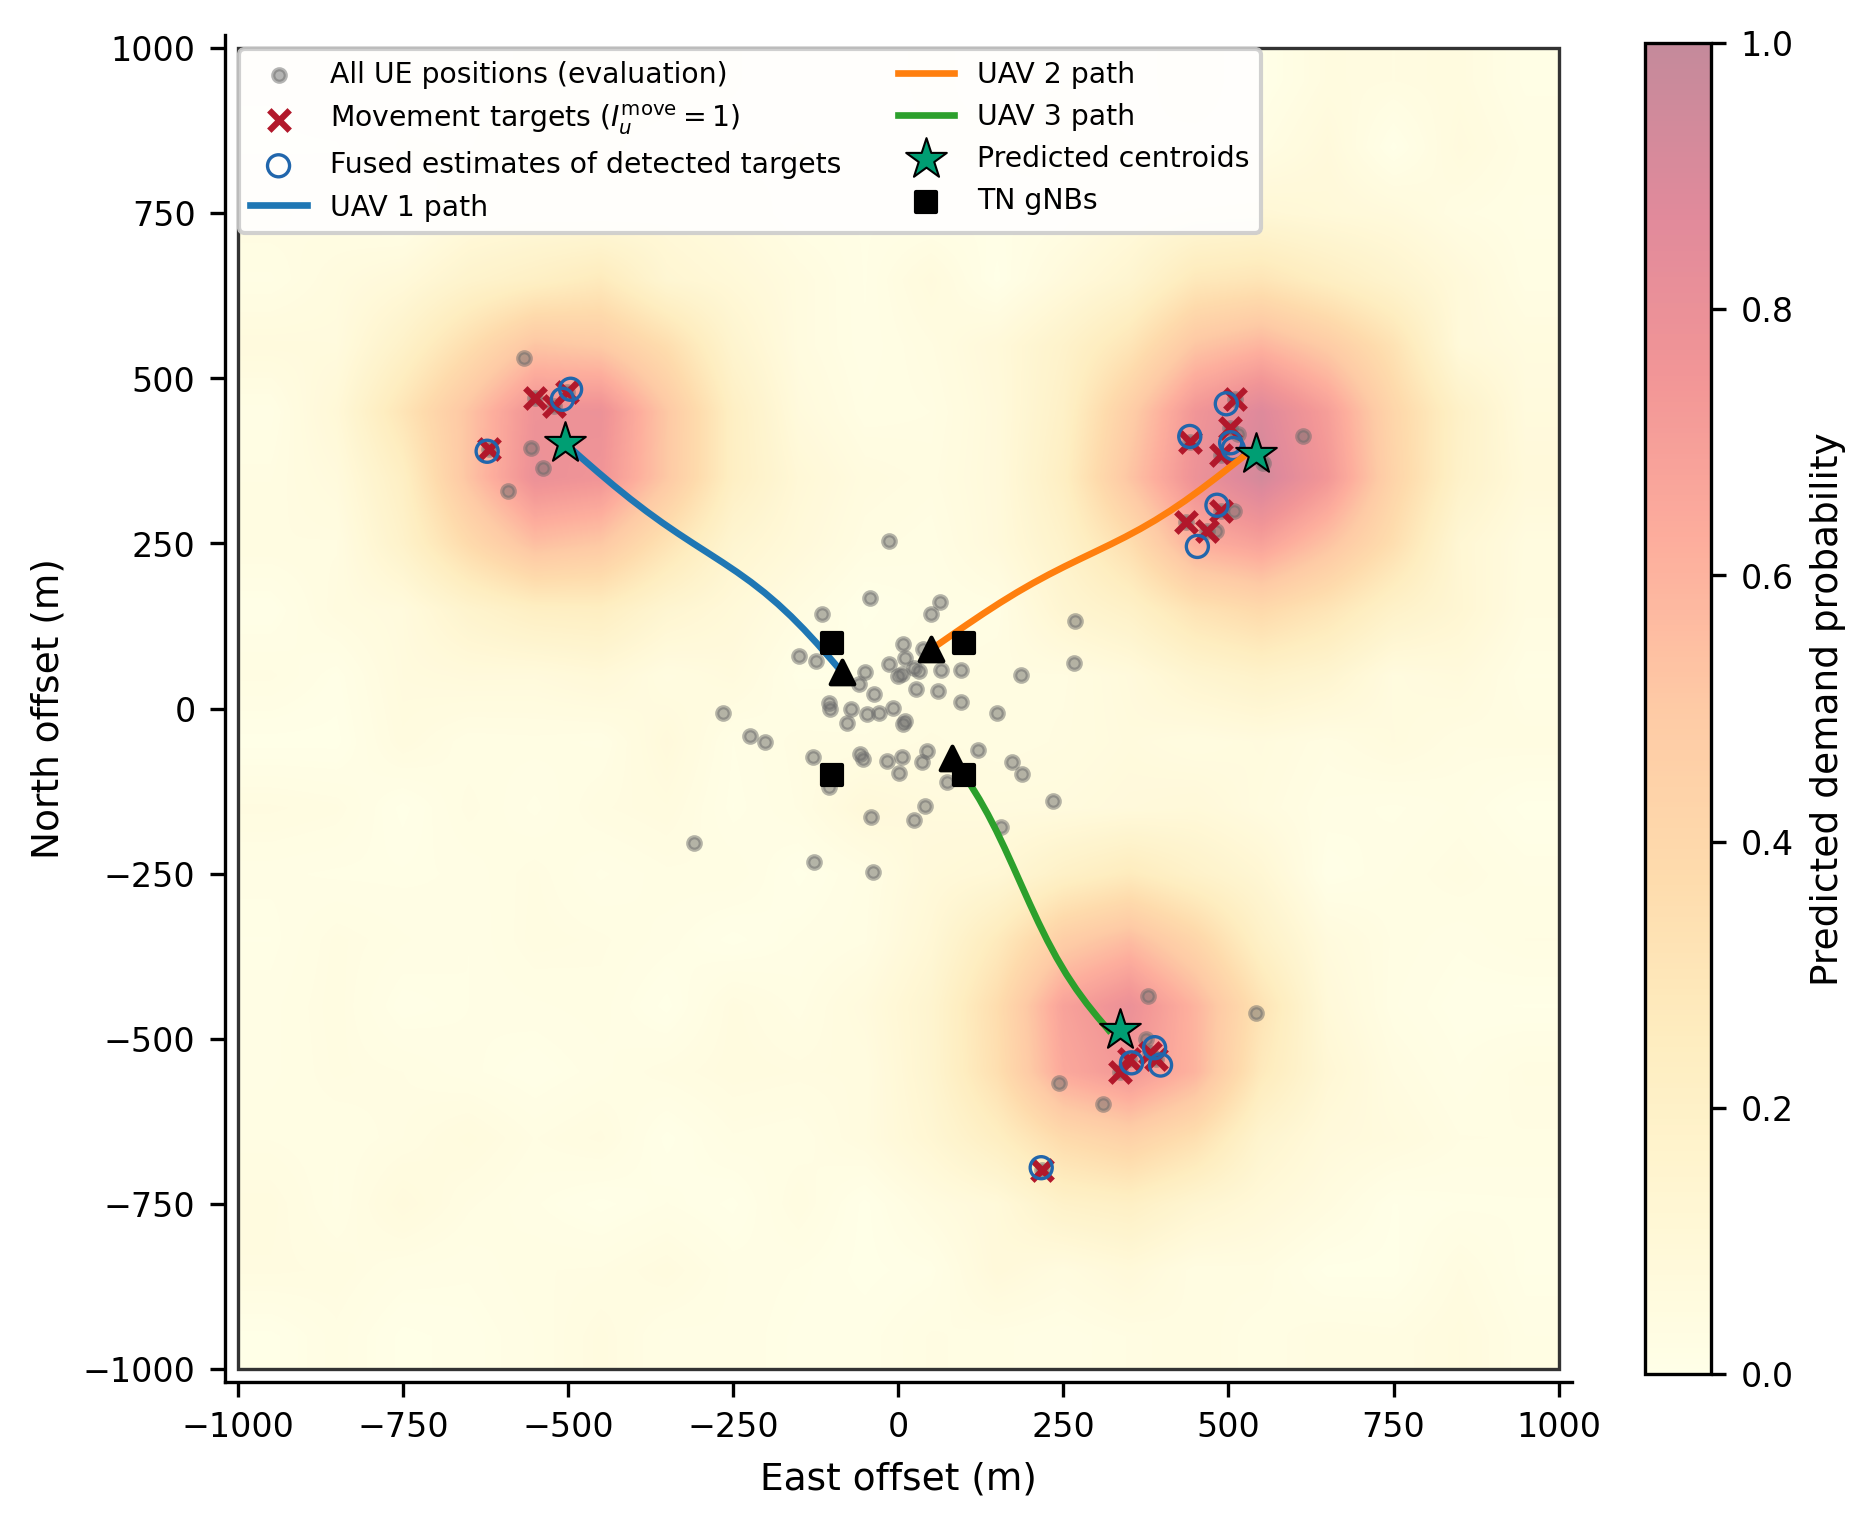
\includegraphics[width=\linewidth]
    {results/plots/sample-png/spatial-repositioning.png}
    \caption{Spatial relationship among all UE evaluation positions,
    movement-target UEs satisfying $I_u^{\mathrm{move}}=1$, fused estimates
    of detected targets, predicted grid-level demand, weighted centroids, and
    UAV trajectories for the synthetic 90-UE example.}
    \label{fig:spatial-repositioning}
\end{figure}
